\documentclass[tikz,border=10pt]{standalone}
\usetikzlibrary{calc}

\begin{document}
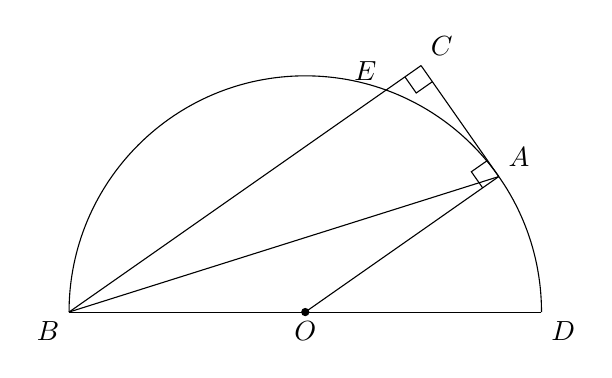
\begin{tikzpicture}
    % Define coordinates
    \coordinate (O) at (0,0);
    \coordinate (B) at (-3,0);
    \coordinate (D) at (3,0);
    
    % Angle alpha = 35 degrees. 
    % This choice ensures OA || BC, which is required by the two right angles.
    \def\alpha{35}
    
    \coordinate (A) at (\alpha:3);
    % E is at angle 2*alpha because triangle OBE is isosceles and angle OBC = alpha
    \coordinate (E) at (2*\alpha:3); 
    
    % C is constructed such that AC is perpendicular to OA (tangent-like) 
    % and AC is perpendicular to BC (given right angle at C).
    % This implies OA || BC.
    % Distance AC = 3*sin(alpha) derived from geometry.
    \coordinate (C) at ($(A) + (\alpha+90:{3*sin(\alpha)})$);
    
    % Draw Semicircle arc
    \draw (B) arc (180:0:3);
    
    % Draw Lines
    \draw (B) -- (D); % Diameter BD
    \draw (B) -- (C); % Line segment BC passing through E
    \draw (A) -- (C); % Segment AC
    \draw (A) -- (B); % Chord AB
    \draw (O) -- (A); % Radius OA
    
    % Right angle at C (between BC and AC)
    % Direction C->B is 180+alpha = 215. Direction C->A is alpha+90+180 = 305.
    \draw ($(C) + (215:0.25)$) -- ($(C) + (215:0.25) + (305:0.25)$) -- ($(C) + (305:0.25)$);
    
    % Right angle at A (between OA and AC)
    % Direction A->O is 180+alpha = 215. Direction A->C is alpha+90 = 125.
    \draw ($(A) + (215:0.25)$) -- ($(A) + (215:0.25) + (125:0.25)$) -- ($(A) + (125:0.25)$);
    
    % Dot at O
    \fill (O) circle (1.5pt);
    
    % Labels
    \node[below left] at (B) {$B$};
    \node[below] at (O) {$O$};
    \node[below right] at (D) {$D$};
    \node[above right] at (A) {$A$};
    \node[above left] at (E) {$E$};
    \node[above right] at (C) {$C$};
    
\end{tikzpicture}
\end{document}
